\section{The Comparison}
\label{sec:new}

As described in the research task C, a parallel implementation is proposed to make inference in a SPN faster.
This parallel solution makes use of a GPU to parallelize computation within each layer.
Since this solution is common to machine learning frameworks, in this implementation TensorFlow is used.
The code is shown below.

\begin{lstlisting}[language=Python]
import numpy as np
from keras.models import Sequential
from keras.layers.core import Dense, Dropout, Layer, Activation
import time
import tensorflow as tf

f = open("results.csv", "w")

for i in range(1,50):

    INPUT_SIZE = 10 * i
    OUTPUT_SIZE = INPUT_SIZE
    nb_class = 3

    batch_size = 128
    nb_epoch = 40

    np.random.seed(123)

    X_train = np.random.rand(INPUT_SIZE, nb_class)
    Y_train = np.random.rand(OUTPUT_SIZE, nb_class)

    X_test = np.random.rand(INPUT_SIZE)
    Y_test = np.random.rand(OUTPUT_SIZE)

    start_time = time.time()

    model = Sequential()
    model.add(Dense(INPUT_SIZE, input_shape=(nb_class,)))
    model.add(Activation('linear'))
    model.add(Dense(OUTPUT_SIZE))
    model.add(Activation('linear'))
    model.compile(loss='categorical_crossentropy', optimizer='rmsprop')

    final_time = time.time()
    diff_time = final_time - start_time

    f.write(str(i)+","+str(diff_time)+","+"\n")

f.close()   
\end{lstlisting}


In the code, we construct a network with 4 layers using random data.
That is, no specific task is being learned by the network.
Then, we perform inference on it during the learning phase.
Also, at each iteration, we increase the size of the input layer, so we can compare the effect of using GPUs as the network gets slightly bigger.
The code is run twice, one with the GPU turned on and another one with it off.
The result is then illustrated in the graph of Figure \ref{fig:graph}.

\begin{figure}[hbt]
    \begin{center}
    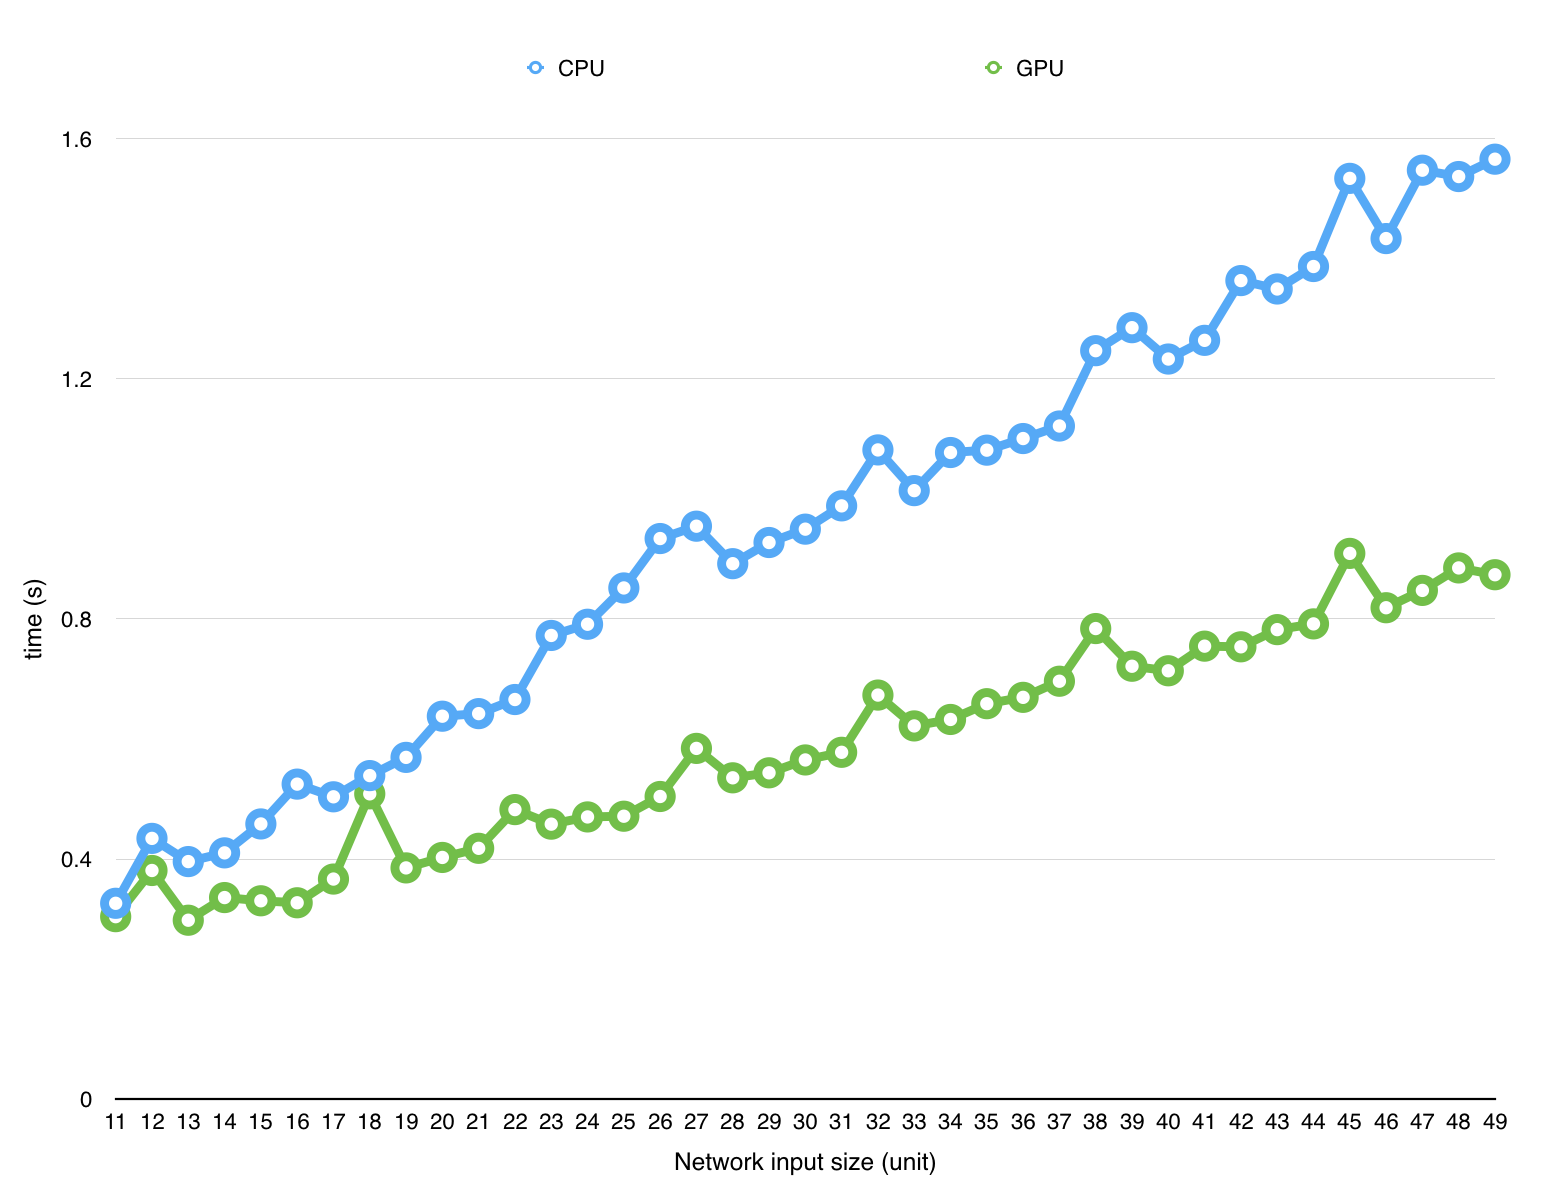
\includegraphics[width=0.8\textwidth]{figures/graph.png}
    \caption{A comparison of inference using a deep network in a GPU and CPU.}
    \label{fig:graph}
    \end{center}
\end{figure}

The graph shows that using GPU makes inference, and therefore learning, faster.
Even when the network gets bigger, using GPU is faster than CPU in a linear fashion.
The peaks in both graph lines can be explained by the non deterministic way that the library creates and manages the networks.
It is worth mentioning that the user only described how the network should be, but the library is the one which creates the network, after using optimization methods.
Therefore, for the randomness of this experiment may cause the performance of these networks to fluctuate as shown in both graphs.
